% Standalone pgfplots: big-Phi inhibition-derivative peak alignment with GZ_LOWER.
% Single-substrate (H_351) vs collective (H_618), against GZ_LOWER = 0.21232.
% Native LaTeX, no Python dep. `make figures` compiles to figures/fig01_inflection_peak.pdf.
\documentclass[border=4pt]{standalone}
\usepackage{pgfplots}
\pgfplotsset{compat=1.18}
\usepackage{amsmath}
\newcommand{\GZL}{\mathrm{GZ_{LOWER}}}
\begin{document}
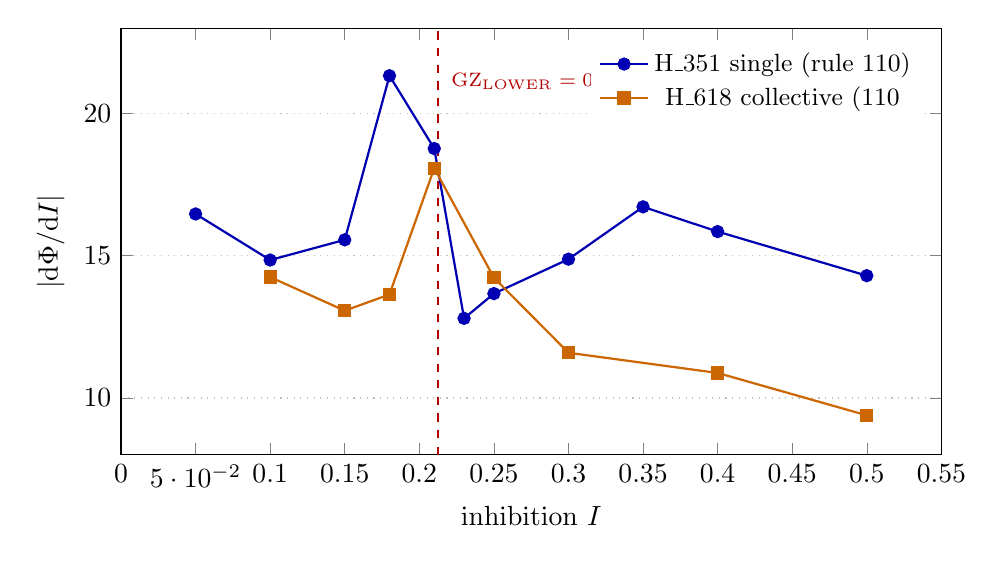
\begin{tikzpicture}
\begin{axis}[
    width=12cm, height=7cm,
    xlabel={inhibition $I$}, ylabel={$|\mathrm{d}\Phi/\mathrm{d}I|$},
    xmin=0.0, xmax=0.55, ymin=8, ymax=23,
    legend style={at={(0.98,0.97)}, anchor=north east, draw=none, font=\small},
    ymajorgrids, grid style={dotted},
]
\addplot[mark=*, blue!70!black, thick] coordinates
  {(0.05,16.47) (0.10,14.85) (0.15,15.56) (0.18,21.33) (0.21,18.77)
   (0.23,12.80) (0.25,13.67) (0.30,14.88) (0.35,16.72) (0.40,15.85)
   (0.50,14.30)};
\addplot[mark=square*, orange!80!black, thick] coordinates
  {(0.10,14.25) (0.15,13.07) (0.18,13.64) (0.21,18.08) (0.25,14.23)
   (0.30,11.59) (0.40,10.88) (0.50,9.39)};
\draw[red!70!black, dashed, thick] (axis cs:0.21232,8) -- (axis cs:0.21232,23);
\node[red!70!black, font=\scriptsize, anchor=south west]
  at (axis cs:0.215,20.5) {$\GZL=0.21232$};
\legend{H\_351 single (rule 110), H\_618 collective (110,110)}
\end{axis}
\end{tikzpicture}
\end{document}
